%------------------------------------------------------------------------------
%   PACKAGES AND OTHER DOCUMENT CONFIGURATIONS
%------------------------------------------------------------------------------

\documentclass[twoside,twocolumn]{article}

\usepackage[english]{babel} % Language hyphenation and typographical rules

% Document margins
\usepackage[hmarginratio=1:1,top=32mm,left=20mm,right=20mm,columnsep=20pt]{geometry}
% Custom captions under/above floats in tables or figures
\usepackage[hang, small,labelfont=bf,up,textfont=it,up]{caption}
\usepackage{booktabs} % Horizontal rules in tables

\usepackage{enumitem} % Customized lists
\setlist[itemize]{noitemsep} % Make itemize lists more compact
\usepackage{textcomp}

% Allows abstract customization
\usepackage{abstract}
% Set the "Abstract" text to bold
\renewcommand{\abstractnamefont}{\normalfont\bfseries}
% Set the abstract itself to small italic text
\renewcommand{\abstracttextfont}{\normalfont\small\itshape}

\usepackage{fancyhdr} % Headers and footers
\pagestyle{fancy} % All pages have headers and footers
\fancyhead{} % Blank out the default header
\fancyfoot{} % Blank out the default footer
\fancyhead[C]{\thetitle}
\fancyfoot[RO,LE]{\thepage} % Custom footer text

\usepackage{titling} % Customizing the title section

\usepackage{hyperref} % For hyperlinks in the PDF
\usepackage{amsmath}

\usepackage{tikz}
\usetikzlibrary{bayesnet}
\usetikzlibrary{arrows}

\usepackage{color}
\usepackage{caption}
\usepackage{subcaption}

\usepackage{graphicx}

\captionsetup[figure]{labelfont={bf},textfont=normalfont}

%------------------------------------------------------------------------------
%   TITLE SECTION
%------------------------------------------------------------------------------

\setlength{\droptitle}{-4\baselineskip} % Move the title up

\pretitle{\begin{center}\Huge\bfseries} % Article title formatting
\posttitle{\end{center}} % Article title closing formatting

\title{Machine Translation Project Proposal: \\ Using Neural Networks to Learn
Word Alignments}
\author{%
\textsc{Bailey Parker} \\[1ex]
\normalsize Johns Hopkins University \\
\normalsize \href{mailto:bailey@jhu.edu}{bailey@jhu.edu}
 \and
 \textsc{Vivian Tsai} \\[1ex]
\normalsize Johns Hopkins University \\
\normalsize \href{mailto:viv@jhu.edu}{viv@jhu.edu}
 \and
  \textsc{William Watson} \\[1ex]
\normalsize Johns Hopkins University \\
\normalsize \href{mailto:billwatson@jhu.edu}{billwatson@jhu.edu}
}

\date{}

%------------------------------------------------------------------------------
\DeclareMathOperator*{\argmax}{arg\,max}
\newcommand{\qdist}[1]{\ifmmode\langle#1\rangle\else\textlangle#1\textrangle\fi}
\renewcommand{\vec}[1]{\mathbf{#1}}

\begin{document}

% Print the title
\maketitle

% \section{Introduction}

% TODO

%------------------------------------------------------------------------------

\begin{abstract}
% \noindent \blindtext
We seek to explore the word alignment problem with the help of neural networks.
More specifically, we want to see if the original Expectation-Maximization
(EM) approach to word alignment can be transcribed as a neural network in both
supervised and unsupervised settings. % add?
\end{abstract}

% REMEMBER: IDEA IS TO COPY PROPOSAL INTO FINAL WRITEUP

%------------------------------------------------------------------------------

\section{Introduction}

% \todo: what is our metric?
Word alignment seeks to match individual words in a parallel corpus such that
the Alignment Error Rate (AER) is minimized. In a previous assignment, we
implemented IBM Model 1, based on the Expectation-Maximization (EM)
algorithm. We then implemented a reparametrization of IBM Model 2 that favors
alignments along the diagonal (\cite{dyer2013simple}). Finally, we implemented an
Alignment by Agreement model (\cite{liang2006alignment}) that trained
French-to-English and English-to-French models and combined the results
to produce better alignments.

Our current proposal is to replace the EM algorithm and
reparametrization of IBM Model 2 with a neural network architecture. Our new
model will additionally incorporate Alignment by Agreement. We will use
PyTorch to build the model and loss functions.

% rephrase sdjfkl
The key concept lies in defining a loss function for which the network will
learn the optimal parameters in order to produce accurate word alignments
from a corpus of parallel text.

%------------------------------------------------------------------------------

\section{Background}

Neural Machine Translation (NMT), particularly attention-based NMT, has
increasingly achieved successful results regarding machine translation tasks
\cite{bahdanau2014neural}. However, the attention mechanisms in neural networks
yield less accurate results than conventional alignment models.
\cite{liu2016neural} and \cite{chen2016guided} have improved upon these results
by using guided alignment training (i.e., supervised training) based on
alignments produced by statistical machine translation
(e.g., fast-align \cite{dyer2013simple}).

% \cite{koehn2019neural} emphasizes the need for an effective alignment
% mechanism between source and target words.

Our approach is inspired by current research in topic modeling with Latent
Dirichlet Allocation (LDA), which is based on variational methods
and EM for Bayes parameter estimation (\cite{blei2003latent}).
\cite{hasler2014dynamic} present a bilingual variant of LDA, called
``phrasal LDA,'' for phrase-based machine translation.

\begin{figure}
\centering
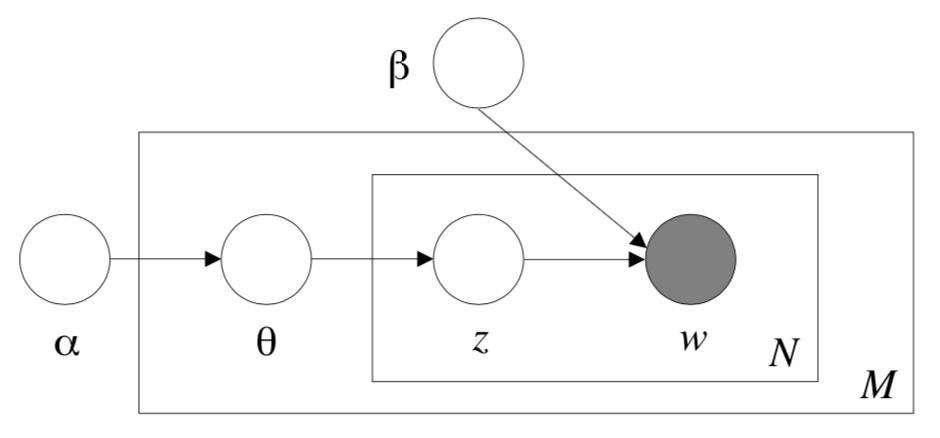
\includegraphics[scale=0.5]{LDADiagram}
% added to description; will probably update later (viv)
\caption{Graphical model representation of LDA from \cite{blei2003latent}, for
topic mixture $\theta$ (for a collection of $M$ documents); set $z$ of $N$
topics; set $w$ of $N$ words, and corpus-level parameters $\alpha$ and $\beta$.
The boxes are ``plates'' representing replicates. The outer plate represents
documents, while the inner plate represents the repeated choice of topics and
words within a document.}
\end{figure}

We additionally draw inspiration from the Autoencoding Variational Bayes (AEVB)
algorithm, particularly as instantiated by the Variational Autoencoder (VAE).
Based on variational inference, AEVB increases efficiency w.r.t. inference and
learning by optimizing a recognition model to approximate posterior
distributions; VAEs use a neural network for this recognition model
\cite{kingma2013auto}.
\cite{srivastava2017autoencoding} present an AEVB-based inference method for
LDA, referred to as Autoencoded Variational Inference for Topic Model (AVITM).

\begin{figure}
\centering
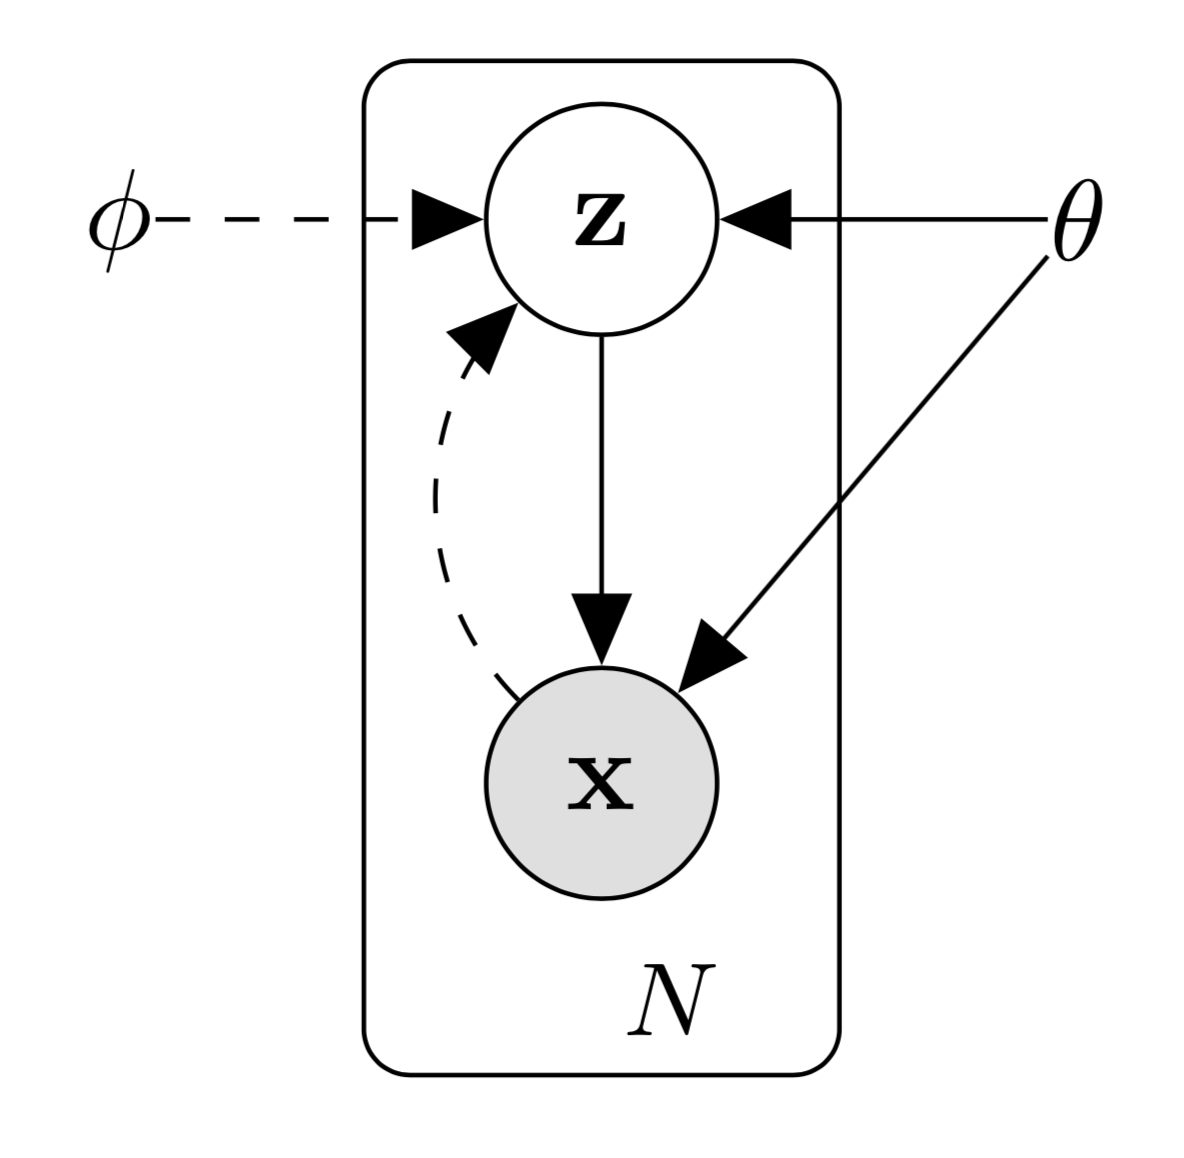
\includegraphics[scale=0.2]{VAEDiagram}
\caption{Graphical model representation of VAE from \cite{kingma2013auto}.
Solid lines denote the generative model $p_\theta(z) p_\theta(x|z)$; dashed
lines denote the variational approximation $q_\phi(z|x)$ to the intractable
posterior $p_\theta(z|x)$. The variational parameters $\phi$ are learned jointly
with the generative model parameters $\theta$.
}
\end{figure}

% VAEs are notable as a popular approach to unsupervised learning and have the
% benefit of being built on neural networks % +trainable via stoch. grad. descent


% LDA models are generative probabilistic models that model topics across
% distributions of words in a corpus. LDAs are based on variational methods
% and EM for Bayes parameter estimation.

% expand this section, and say that the work is inspiration to our approach
% applying a NN to approximate the posterior distributions.
% see apibm - apply tech to lda.

% Current research attempts to supplant the probabilistic modeling with a
% neural network architecture.


%------------------------------------------------------------------------------

\section{Original Formulation}
\label{sec:original-formulation}
% \todo: shorten or rephrase

IBM Model 1 estimates the translation probabilities of the data through the EM
algorithm
\footnote{\url{http://mt-class.org/jhu/assets/papers/alopez-model1-tutorial.pdf}},
which is useful in discovering and learning the parameters of a
latent variable model.
In the original IBM Model 1, we define the translation probability distribution
as $\tau(t_i|s_j)$ for target word $t_i$ and source word $s_j$.

Dyer et al. \cite{dyer2013simple} added an effective reparameterization
of IBM Model 2 to produce alignment distribution $a$. We define (for a source
(French) sentence \textbf{s} of length $n = |\textbf{s}|$ and a target (English)
sentence \textbf{t} of length $m = |\textbf{t}|$, with precision parameter
$\lambda$) this alignment distribution $a$ as follows:

\begin{equation}
\begin{split}
h(i,j,m,n) = - \left| \frac{i}{m} - \frac{j}{n}\right| \\
\\
a(i,j,m,n) =e^{  \lambda h(i,j,m,n)} \\
\end{split}
\end{equation}

This formulation gives us a positionally-aware distribution that favors alignments
towards the diagonal for a given source word $t_i$ and target word $s_j$. The
precision parameter $\lambda$ controls how strongly the model prefers the
diagonal.

Once we are done training the model, to make an alignment guess, we must find
the alignment that returns the maximum probability. For some alignment $a_i$:
\begin{equation}
\hat{a}_i = \argmax_{a_i} \, \tau(t_{a_i}|s_j) \cdot a(i, j, m, n)
\end{equation}
where $\tau(t_{a_i}|s_j)$ is the translation probability, and an alignment
distribution $a$ with parameters $\lambda$ and $p_0$. This will give us the
English word $t_{a_i}$ that is the most likely translation of the French word
$s_j$.

Finally, incorporating the Alignment by Agreement model improvement was
inspired by the work done by Liang et al. \cite{liang2006alignment}. However,
our original implementation was strongly influenced by the pseudocode used in
the \texttt{Grow-Diag-Final} Alignment Heuristic by the Moses Statistical
Translation
System\footnote{\url{http://www.statmt.org/moses/?n=FactoredTraining.AlignWords}}.

We trained an EM model in both directions, one for source-to-target
(English-to-French), $A_{S \rightarrow T}$, and another for target-to-source
(French-to-English), $A_{T \rightarrow S}$.
Using the alignments generated by each individual model, we then took the intersection of each model's alignments. This effectively gave an alignment
matrix that both models favored strongly (i.e., agreed on).

%\begin{equation}
%\text{Intersection} = A_{S \rightarrow T} \, \bigcap \, A_{T \rightarrow S}
%\end{equation}
%\begin{equation}
%\text{Union} = A_{T \rightarrow S} \, \bigcup \, A_{S \rightarrow T}
%\end{equation}

From our intersection matrix, we then used the \texttt{GROW-DIAG-FINAL}
algorithm to fill in the remaining gaps from the union of alignments.

\begin{figure}
\centering
\begin{tikzpicture}

  % Define nodes
  \node[obs]                               (t) {$t$};
  \node[latent, above=0.75cm of t] (a) {$a$};
  \node[latent, above=0.75cm of a, xshift=-0.6cm] (lambda) {$\lambda$};
  \node[latent, above=0.75cm of a, xshift=0.6cm]  (null) {$p_0$};
  \node[obs, right=0.75cm of t]            (s) {$s$};
  \node[latent, below=0.95cm of t]            (theta) {$\theta$};

  % Connect the nodes
  \edge {null,lambda} {a} ; %
  \edge {a,s, theta} {t} ; %

  % Plates
  \plate [xscale=1.75, yscale=1.25] {t} {(a)(t)} {$\quad$} ;

\end{tikzpicture}
\caption{Our probabilistic plate diagram for word alignment, where $t$ is
target, $s$ is source, $\theta$ is the translation model, $\lambda$ is a
position distortion parameter, $p_0$ is the null probability, and $a$ is the
alignment distribution.}
\end{figure}

%------------------------------------------------------------------------------

% talk about NN formulation, see hand notes
\section{Neural Network Architecture}

We describe our model architecture to learn word alignments, along with
a combined loss function that will encode alignment by
agreement for both source-to-target and target-to-source embeddings.

% \todo: needs work (says Achintya, via text)

\subsection{Model Description}

Our model will consist of two parts: the pseudo E-Step prediction network, and
the pseudo M-Step evaluation (loss) function.

This prediction network accepts two inputs: a target sentence $t$ and a source
sentence $s$. The network outputs an alignment matrix $\psi$, where
each row corresponds to a source word $s_i$ and each column corresponds to a
target word $t_j$. This will help in consistency of future operations.

\begin{equation}
  \centering
\begin{array}{c|ccccc}
\psi & t_1       & \hdots & t_j       & \hdots & t_m       \\ \hline
s_1  & \psi_{11} & \hdots & \psi_{1j} & \hdots & \psi_{1m} \\
\vdots  & \vdots & \ddots & \vdots &  & \vdots \\
s_i  & \psi_{i1} & \hdots & \psi_{ij} & \hdots & \psi_{im} \\
\vdots  & \vdots &  & \vdots & \ddots & \vdots \\
s_n  & \psi_{n1} & \hdots & \psi_{nj} & \hdots & \psi_{nm}
\end{array}
\end{equation}

The prediction network mimics the E-Step by learning alignments and outputting
a $\psi$ matrix that can be thought of as a similarity matrix for every target
word $t_j$ and source word $s_i$.

We define the length of the target sentence
$|t| = m$ and the length of the source sentence as $|s|=n$. Hence the $\psi$
matrix is an $n \times m$ matrix containing measures of similarity between each
$j$-th target word and $i$-th source word.

We have several ideas on how to generate this alignment matrix $\psi$:
\begin{enumerate}
  \item Given target word embedding $W_t$ and source word embedding $W_s$,
  take the element-wise dot product. Then for each $t_j$, $s_i$ pairing:
  \begin{equation}
    \psi_{ij} = W_t[t_j] \cdot W_s[s_i]
  \end{equation}
  \item Use word embeddings and bi-directional LSTMs to generate alignment
    matrix $\psi$ that considers the whole sequence for both sentences.
  \item Explore deeper, more complex architectures to create a $n \times m$
    alignment matrix $\psi$.
\end{enumerate}

\begin{figure}
\centering
\begin{tikzpicture}

  % Define nodes
  \node[latent] (psi) {$\psi$};
  \node[latent, above=0.95cm of psi] (a) {$a$};
  \node[obs, above=0.85cm of a, xshift=-0.6cm] (t) {$t$};
  \node[obs, above=0.85cm of a, xshift=0.6cm] (s) {$s$};
  \node[latent, below=0.75cm of psi] (p) {$-\log p(t, s | \theta, \psi)$};
  \node[latent, left=0.75cm of p] (kl) {$D_{\mathrm{KL}} ( \sigma_t(\psi) \| a_t)$};
  \node[latent, right=0.75cm of psi] (theta) {$\theta$};
  \node[latent, below=0.95cm of p] (sum) {$\Sigma$};
  \node[latent, below=0.95cm of sum] (loss) {$Loss$};

  % Connect the nodes
  \edge {t,s} {a} ; %
  \edge {a} {psi} ; %
  \edge {psi} {kl} ; %
  \edge {psi, theta} {p} ; %
  \edge {p, kl} {sum} ; %
  \edge {sum} {loss} ; %

  % Plates
  \plate [yscale=1.25, yshift=.1cm] {t} {(a)} {} ;

\end{tikzpicture}
\caption{Model Architecture for source $s$ to target $t$ alignments. Neural
network alignment model $a$ generates alignment matrix $\psi$. $\theta$ are
learnable translation probabilities. Evaluation function
$- \log p(t, s | \theta, \psi)$ and KL Divergence $D_{\mathrm{KL}}$ produce our
loss function (to be minimized).}
\end{figure}


\subsection{Loss Function}

To create our loss function, we convert our alignment matrix $\psi$
to a probability distribution. We define $\sigma(\vec{x})$ as
the softmax operator applied on vector $\vec{x}$, and $\sigma(\vec{x})_i$ as
the $x_i$ softmax probability for vector $\vec{x}$.

\begin{equation}
\sigma(\vec{x})_i = \frac{\exp(x_i)}{\sum_j\exp(x_j)}
\end{equation}

We therefore define two operations on the alignment matrix $\psi$. For source
$s$ to target $t$ probability generations, we define $\sigma_t(\psi)$ as the
softmax on each column, i.e., target word $t_j$.
\begin{equation}
  \sigma_t(\psi) = \left[
    \begin{matrix}
      \sigma(\psi_{t_1}) &
      \hdots &
      \sigma(\psi_{t_j}) &
      \hdots &
      \sigma(\psi_{t_m})  \\
    \end{matrix}
\right]
\end{equation}

In addition, we further define the target-to-source generation as
$\sigma_s(\psi)$, where the softmax operator is applied on each row for target
word $s_i$ and produces a row vector.
\begin{equation}
  \sigma_s(\psi) = \left[
    \begin{matrix}
      \sigma(\psi_{s_1})  \\
      \vdots \\
      \sigma(\psi_{s_i})  \\
      \vdots \\
      \sigma(\psi_{s_n})  \\
    \end{matrix}
\right]
\end{equation}

While VAEs sample from the probability distribution derived by the neural
network, our model's distribution is discrete. Therefore, we need not
sample and can instead compute the loss in terms of all possibilities.

The following subsections describe our loss functions:

\subsubsection{Probability Maximization}

In our original formulation (Section \ref{sec:original-formulation}), we
maximized probabilities for word alignments.
For this model, we define $p(t, s | \theta, \psi)$ as such:

\begin{equation}
  \begin{split}
  p(t, s | \theta, \psi)
    &= \prod_j^{|t|} \sum_i^{|s|} p_\theta(t_j| s_i) \cdot p_a(i|j) \\
    &= \prod_j^{|t|} \sum_i^{|s|} \sigma_s(\theta(t_j, s_i)) \cdot \sigma_t(\psi)_{ij}
  \end{split}{}
\end{equation}

This formula stems from our assumption that the alignments for each
target word are conditionally independent, hence a product over target
words $t_j$. We then sum over all the alignment possibilities from the source
words $s_i$, thus marginalizing over the alignments.

For $s \mapsto t$ alignments, alignments are softmaxed per column becuase we hold the target $t$ constant and iterate over the source $s$, hence $\sigma_s$.

The translation probabilities are softmaxed per row (i.e., source word $s_i$) since we are given a source word
and want to know the probability of translating $s_i$ to $t_j$, hence $\sigma_t$.

However, as we do not maximize in neural networks, we must transform this
equation into a minimization problem by taking the negative log of $p$:

\begin{equation}
  \begin{split}
  -\log p(t, & s | \theta, \psi) = \\
  - \sum_j^{|t|}
    & \log \left[ \sum_i^{|s|} \sigma_s \left( \theta(t_j, s_i) \right) \cdot
      \sigma_t(\psi)_{ij} \right]
\end{split}
\end{equation}

We can simplify this into the equation below, for easier implementation
(via PyTorch's \texttt{logsumexp} function):

\begin{equation}
  \centering
  \begin{split}
  -\log  p(t & , s | \theta, \psi) = \\
  - \sum_j^{|t|} & \log \left[ \sum_i^{|s|} \exp
      \left( \log \sigma_s(\theta(t_j, s_i)) + \log \sigma_t(\psi)_{ij} \right)
    \right]
\end{split}
\end{equation}

This is the term to be minimized for our source-to-target word alignment
generation.


\subsubsection{KL Divergence and Prior Terms}

We also need to minimize the Kullback-Leibler (KL) divergence between our
distribution and a prior. For discrete probability distributions $P$ and $Q$
defined on the same probability space, the reverse KL divergence from $Q$ to
$P$ is defined as:

\begin{equation}
D_{\mathrm{KL}}(Q \| P) = \sum_{i} Q(i) \log \left( \frac{Q(i)}{P(i)} \right)
\end{equation}

In other words, it is the expectation of the log difference between the
probabilities $P$ and $Q$, where the expectation is taken using the
probabilities $Q$.

To calculate the KL divergence of our model, we must define
distributions $P$ and $Q$. We first consider $P$ as our prior
distribution, henceforth called $a_t$. This prior distribution $a_t$ is a
$n \times m$ matrix filled with the alignment probabilities filled for source
word $s_i$; target word $t_j$; source sentence $s$ of length $n$; and target
sentence $t$ of length $m$:

We define distortion exponent $h$ as:
\begin{equation}
  h(i, j) = {-\lambda \left| \frac{i}{n} - \frac{j}{m}\right|}
\end{equation}

% might have to flip this to be sum over i' not j' DONE
\begin{equation}
  Z_j = \sum_{i'} \exp h(i', j)
\end{equation}

\begin{equation}
a_t (i, j) =
\begin{cases}
      p_0 & \text{if } null \\
     (1-p_0) \cdot \frac{e^{h(i,j)}}{Z_j} & \text{else}
   \end{cases}
\end{equation}

In \cite{dyer2013simple}, parameter values were selected as
$\lambda = 4$ and $p_0 = 0.08$ for the entire corpus.
Each element value of $a_t$ is normalized by the sum of the column distortion
values to create a valid distribution via term $Z_j$ (since we hold target $t_j$ constant). For future notation, let the subscript on the distirbution $a$ denote
the way we normalize; i.e., $a_t$ is the prior alignment distribution normalized
with respect to target words $t_j$ and thus normalized by the sum of the column
for $t_j$.

% \todo: change?
We can then write our KL Divergence (to be minimized) as:

\begin{equation}
  D_{\mathrm{KL}}(\sigma_t(\psi) \| a_t) =
    \sum_i^n \sum_j^m \sigma_t(\psi)_{ij} \cdot
      \log \left[ \frac{\sigma_t(\psi)_{ij}}{a_t(i, j)} \right]
\end{equation}


\subsubsection{Target-to-Source Loss Terms}

We have described the loss terms for a source $s$ to target $t$ word alignment.
However, we seek to perform alignment by agreement. Hence, we must add loss
functions that describe the evaluation of target $t$ to source $s$:

\begin{equation}
  \centering
  \begin{split}
  -\log  p(t & , s | \theta, \psi) = \\
  - \sum_i^{|s|} & \log \left[ \sum_j^{|t|}
      \exp \left(
        \log \sigma_t(\theta(t_j, s_i)) + \log \sigma_s(\psi)_{ij}
      \right)
    \right]
\end{split}
\end{equation}

\noindent
Additionally, for the KL Divergence term for target $t$ to source $s$:

\begin{equation}
D_{\mathrm{KL}} (\sigma_s(\psi) \| a_s) = \sum_i^n \sum_j^m \sigma_s(\psi)_{ij}
  \cdot \log \left[ \frac{\sigma_s(\psi)_{ij}}{a_s(i, j)} \right]
\end{equation}

\noindent
where the normalization of the prior $a_s$ is on the row instead of the column.
In other words, we hold the source $s_i$ constant; sum the row; and divide each
row element by the sum.

The equations for $a_s$ are as follows:

\begin{equation}
  h(i, j) = {-\lambda \left| \frac{i}{n} - \frac{j}{m}\right|}
\end{equation}

% might have to flip this to be sum over i' not j' DONE
\begin{equation}
  Z_i = \sum_{j'} \exp h(i, j')
\end{equation}

\begin{equation}
a_s (i, j) =
\begin{cases}
      p_0 & \text{if } null \\
     (1-p_0) \cdot \frac{e^{h(i,j)}}{Z_i} & \text{else}
   \end{cases}
\end{equation}

We also perform the softmax operator on each column of the $\psi$ matrix,
previously defined as $\sigma_t(\psi)$.


\subsubsection{Alignment by Agreement}

Finally, one last loss function term must be added to jointly train each model.
We define $\circ$ as the Hadamard Product, which is the element-wise
multiplication of two matrices. For instance:
$(A \circ B)_{ij} = A_{ij} \cdot B_{ij}$.

We can write the term as such:

\begin{equation}
  -\log \sum_i^{|s|} \sum_j^{|t|}
    \left[ \sigma_s(\psi) \circ \sigma_t(\psi) \right]_{ij}
\end{equation}

% Again note here, you can use logsumexp trick to implement this efficiently in
% PyTorch


\subsubsection{Combined Loss Function}

Our final loss function, to be minimized, is a 5-term equation. We define:
\begin{itemize}[label={}]
  \item $a_t$ as the target prior alignment matrix normalized per column with respect to $t$\\ %per col wrt t
  \item $a_s$ as the source prior alignment matrix normalized per row with respect to $s$\\ %per row wrt s
  \item $\sigma_s$ as the softmax operator applied on the rows of a matrix\\
  \item $\sigma_t$ as the softmax operator applied to each column of a matrix
\end{itemize}

Indexing is done under the assumption that source words $s_i$ form rows
and target words $t_j$ form columns. The term $ij$ is a shorthand
for $s_i$ and $t_j$ indexing into our matrices.

\begin{equation}
  \centering
\begin{split}
  Lo&ss = \\
  &- \sum_j^{|t|} \log \left[
      \sum_i^{|s|} \exp \left(
        \log \sigma_s(\theta(t, s))_{ij} + \log \sigma_t(\psi)_{ij} \right)
    \right] \\
  &+ \sum_i^n \sum_j^m \sigma_t(\psi)_{ij} \cdot \log \left[
    \frac{\sigma_t(\psi)_{ij}}{a_t(i, j)} \right] \\
  &- \sum_i^{|s|} \log \left[ \sum_j^{|t|}
      \exp \left(
        \log \sigma_t(\theta(t, s))_{ij} + \log \sigma_s(\psi)_{ij}
      \right)
    \right] \\
  &+ \sum_i^n \sum_j^m \sigma_s(\psi)_{ij} \cdot \log \left[
    \frac{\sigma_s(\psi)_{ij}}{a_s(i, j)} \right] \\
  &- \log \sum_i^{|s|} \sum_j^{|t|} \left[
    \sigma_s(\psi) \circ \sigma_t(\psi) \right]_{ij} \\
\end{split}
\end{equation}

% Note, the alignment prior is not exactly the same for source-to-target and
% target-to-source because even though the loss function is symmetric, the
% probabilities are normalized with respect to n or m, depending which
% direction you are translating


\subsection{Prediction}

For prediction, we can set a threshold for our alignment matrix $\psi$ and
return all alignments above this threshold.

%------------------------------------------------------------------------------

\section{Data}

% talk about subtitle extraction. Also labeling of data for supervised? Or
% should that go in supervised training section. Get Bailey to mention Nikita
% metric for baseline on unaligned corpus.


\subsection{Introduction}

The efficacy of a neural network alignment system depends heavily on the
quantity and quality of the training data available. We look to leverage
existing corpora of natural language in various settings instead of the
traditional corpora (such as Europal, which is domain-specific and lacks the
unstructured and informal nature of everyday language). Training on these
commonly-used corpora leads to models with preferences for emitting language
of a parliamentary nature; we elect to focus on corpora that
provide more of a contextual breadth.

To this end, we amassed a corpus of domestic and international movie and TV
show subtitles from a variety of sources. Subtitles have the unique advantage
of being already sentence-aligned, thanks to timestamps. This alignment
somewhat holds even if timestamps are skewed between different media
formats of the same source with slightly different timings.

Our preference was to collect only professional or official subtitles, but
unfortunately these fall under copyright law and are often not publicly
available. However, there are communities of volunteer transcribers and
translators from which we can obtain unofficial subtitles. Many of these
communities have databases with publicly available dumps of all translations,
offer an API, or have a website that is scrapeable. We have employed these
tactics to obtain an initial corpus (see
\hyperref[subsec:procuring-subtitles]{Procuring Subtitles}).

We plan to handle subtitles in strict alignment (that is, those whose timestamps
correspond exactly) and will also attempt to sentence-align those in
fuzzy alignment (i.e., timestamps do not correspond one-to-one). For more on our
methodology, see \hyperref[subsec:subtitle-alignment]{Subtitle Alignment}.

For evaluating the effectiveness of our model and to facilitate
supervised training, we require ground truth alignments for some subset of our corpus. As our corpus currently has 90 million English-French aligned subtitles
(each approximately consisting of one sentence), it impractical to align by hand,
even with significant resources.
We are thus presented with an evaluation problem similar to that in Liu et al.
\cite{liu2015streaming} (though instead of the ground truth being intractable,
our ground truth is impractical to compute).

We elect to obtain ground truth alignments by a consensus-based
approach similar to that in \cite{liu2015streaming}. Broadly, we look to
well-known open-source alignment software \textit{en masse} to provide an approximation of the ground truth alignments.
We do so by evaluating the pairwise overlap between
each aligner and our model to determine a metric that can approximate
Alignment Error Rate (AER) (see
\hyperref[subsec:ground-truth-alignments]{Ground Truth Alignments}).

\subsection{Procuring Subtitles}
\label{subsec:procuring-subtitles}

Subtitles were procured via a variety of means, including downloading data
dumps; using APIs; and web scraping.

Websites like \href{https://www.opensubtitles.org/}{OpenSubtitles} offer
open source tarballs of their available subtitles. We obtained
a recent version of this dump and have begun tooling to massage it into a
uniform format so that we can import it into our corpus.

Communities like the aforementioned, while operating in a legal gray area, tend
to be on the up-and-up in that they respond to DMCA takedown requests. Other
websites adhere to these with less urgency, so we elect not to link them.
However, these sites are still useful communities of tens of thousands of
transcribers and translators whose subtitles can be useful for our corpus.

Due to their underground nature, many of these sites place strict download
limits on subtitles. To combat this, we engineered tools to cleverly extract metadata (by utilizing a breadth of different-DC hosts doing intelligent
scraping); we then make intelligent decisions on which subtitles to procure,
based on quality metrics computed from this metadata. These metrics include user subtitle rating (if available); number of downloads (normalized per
movie/episode); and number of editors/edits. The metrics can also be normalized across language, as certain languages have more subtitles than others.

Other websites avoid the legal gray area of hosting subtitles and translations
by employing deniability tactics, such as requiring the SHA256 hash of a video
file (instead of a movie title or show name) to locate subtitles. Such sites
include \href{http://thesubdb.com/}{SubDB}, which provides an open API for
accessing subtitles. We are currently exploring methods for collecting lists of
hashes of popular media (by scraping websites which list this media) that we
can feed through this website. This would have the twofold advantage of
i) allowing us to index their database for subtitles in which we are interested
and ii) giving us subtitle alignments to other sources. We also considered
reaching out to the owners of such databases, but since they only maintain
hashes, we would still need a way of associating subtitles with their source
media.


\subsubsection{Unified Data Format}

As a secondary step to procurement, we need to unify the disparate data
collected from various sources into a format that allows us to make decisions
about language pairs and easily extract pairable subtitle files for alignment.
For this purpose, we wrote custom scripting utilities for i) parsing
the data formats obtained from each of the source websites and ii) converting
all relevant data into a unified, compact binary format that is designed to be
streamed. This format allows for online streaming creation from a live stream
of incoming data and also permits out-of-memory statistical analysis and
subtitle file alignment.


\subsection{Subtitle Alignment}
\label{subsec:subtitle-alignment}

We have two goals in data processing. First, we must align
subtitle files from matching shows and episodes within sources and between
sources. Then, once we have pairs of subtitle files (each of the same medium,
but translated into different languages), we can begin the next step of
tokenizing and aligning their sentences to produce appropriate input for
our model. We can also use these pairs to derive
\hyperref[subsec:ground-truth-alignments]{Ground Truth Alignments} for the
purposes of model evaluation and supervised training.

We have several cases of subtitle file alignment to consider. Suppose we have
Subtitle file \textit{A} (in language \textit{S}) and Subtitle file \textit{B}
(in language \textit{T}). Then we have

\begin{enumerate}

    \item Files \textit{A} and \textit{B} are from the same source. Further,
        the files were grouped together on their source website under the same
        translation version. This means that one is a derivative/translation
        of the other. This can be confirmed by examining the number of lines
        in each file (and the timestamps of the subtitles). Typically these
        files are in one-to-one or near-one-to-one correspondence. We call
        these files ``exact pairs.'' Producing aligned sentences from these is
        trivial. Simply traverse the two in lock step and each each sentence
        pair you encounter.

    \item Files \textit{A} and \textit{B} are from the same source. However,
        while they are for the same medium, they aren't grouped under the
        same subtitle version. This means they may not be derivatives of
        one another (for example, they may have been independently transcribed
        and translated solely by watching the source material instead of
        consulting another subtitle). We call \textit{A} and \textit{B} a
        ``fuzzy pair.'' This case is slightly more complex to handle, because
        \textit{A} and \textit{B} may have been transcribed from different
        media formats with different timing delays. However, sentence
        alignments can still be produced by taking advantage of the fact that
        their sequential nature is still preserved. By employing some
        heuristics and interpolation, we can generate high-certainty sentence
        pairings. We plan to evaluate these pairings by analyzing in isolation
        the AER on this dataset when fed through the software we plan to use
        for \hyperref[subsec:ground-truth-alignments]{Ground Truth Alignments}.

    \item Files \textit{A} and \textit{B} are from different sources. This can
        largely be treated the same as the case above, however we first must
        determine if \textit{A} and \textit{B} are subtitles for the same media
        in different languages. We have metadata identifying languages
        \textit{S} and \textit{T} and the files, so eliminating same-language
        pairs is trivial. To match media, we employ NLP techniques to perform
        fuzzy matching on file metadata in an attempt to correlate movie/show
        title, episode/season name/number, etc. We may also consult an external
        metadata database to unify our subtitle metadata.

\end{enumerate}

Considerations must also be made to perform the aforementioned processes
efficiently, due to large corpus size.

Another consideration we plan to make is ensuring that from the breadth of
sources we don't produce duplicate subtitle pairings (if, for example, two
sources provided the exact same subtitles). This will likely consist an
extra post processing step before the data is given to the alignment model for
training.


\subsubsection{Preliminary Corpus Statistics}

We briefly summarize statistics on a subset of our corpus, which has already
been collected and processed by the data unification pipeline. A
significant portion of our corpus has been withheld from these numbers as it
is still processing. Additionally, we plan to collect data from even more
sources to negate any effects of average quality subtitles.

Looking at language prevalence, we have 84,000 English subtitle files and
23,000 French subtitle file (Figure \ref{fig:language-prevalence}). We note
that each file contains many sentences.

\begin{figure}[ht]
    \centering
    \begin{tabular}{ |l|r| }
        \hline
        \multicolumn{1}{|c|}{\textbf{Language}} &
            \multicolumn{1}{|c|}{\textbf{Subtitle Files}} \\
        \hline
        English    & 84,959 \\  \hline
        French     & 23,195 \\  \hline
        Portuguese & 16,912 \\  \hline
        Italian    & 15,998 \\  \hline
        Dutch      & 10,690 \\  \hline
        Spanish    & 10,515 \\  \hline
        German     & 5,462  \\  \hline
        Romanian   & 4,726  \\  \hline
        Bulgarian  & 3,136  \\  \hline
        Greek      & 2,246  \\  \hline
    \end{tabular}

    \caption{Number of subtitle files for the top 10 most prevalent langauges
             in our corpus subset}
    \label{fig:language-prevalence}
\end{figure}

Next, we note the approximate number of sentence pairs per ``exact pair" of
subtitle languages (Figure \ref{fig:exact-pair-sentences}). There
are a significant number (5.7 million) of already aligned sentences for
English, French. However, we'd like more data than this, so we also consider
``fuzzy pairs" (Figure \ref{fig:fuzzy-pair-sentences}).

When considering ``fuzzy pairs" in addition to the ``exact pairs" we see that
we now have a plethora of sentence pairs. Notably, we have over 80 million
English-French sentence pairs and 67 million English-Italian sentence pairs.
We also have mobility between language pairs that don't include English
(55.6 million French-Italian sentence pairs, for example). Such a large corpus
of pairs allows us to comfortably train and evaluate the alignment model on
various language pairs to determine its efficacy.

\begin{figure}[ht]
    \centering
    \begin{tabular}{ |l|r| }
        \hline
        \multicolumn{1}{|c|}{\textbf{Exact Language Pair}} &
            \multicolumn{1}{|c|}{\textbf{Aligned Sentences}} \\ \hline
        English, French       & 5,747,845 \\ \hline
        English, Bulgarian    & 1,918,850 \\ \hline
        French, Bulgarian     & 1,115,980 \\ \hline
        English, Portuguese   & 754,248   \\ \hline
        French, Portuguese    & 404,377   \\ \hline
        English, Spanish      & 340,123   \\ \hline
        Portuguese, Bulgarian & 211,751   \\ \hline
        English, Romanian     & 160,416   \\ \hline
        English, Greek        & 120,561   \\ \hline
        French, Romanian      & 87,082    \\ \hline
    \end{tabular}

    \caption{Top 10 approximate number of sentence pairs per ``exact pair" of
             subtitle languages}
    \label{fig:exact-pair-sentences}
\end{figure}

\begin{figure}[ht]
    \centering
    \begin{tabular}{ |l|r| }
        \hline
        \multicolumn{1}{|c|}{\textbf{Fuzzy Language Pair}} &
            \multicolumn{1}{|c|}{\textbf{Aligned Sentences}} \\
        \hline
        English, French     & 81,627,311 \\ \hline
        English, Italian    & 67,458,538 \\ \hline
        Italian, French     & 55,623,242 \\ \hline
        English, Portuguese & 55,487,067 \\ \hline
        French, Portuguese  & 43,822,977 \\ \hline
        English, Dutch      & 41,648,439 \\ \hline
        English, Spanish    & 39,650,085 \\ \hline
        Italian, Portuguese & 36,098,391 \\ \hline
        French, Dutch       & 35,809,672 \\ \hline
        English, German     & 32,495,335 \\ \hline
        Spanish, French     & 31,086,831 \\ \hline
        Italian, Dutch      & 29,880,240 \\ \hline
        French, German      & 27,358,847 \\ \hline
        Portuguese, German  & 26,362,749 \\ \hline
        Spanish, Italian    & 26,182,558 \\ \hline
        Italian, German     & 23,596,809 \\ \hline
        Spanish, Portuguese & 23,451,001 \\ \hline
        English, Romanian   & 22,800,267 \\ \hline
        Portuguese, Dutch   & 21,380,712 \\ \hline
        English, Bulgarian  & 20,239,688 \\ \hline
    \end{tabular}

    \caption{Top 20 number of approximate sentence pairs per ``fuzzy pair" of
             subtitle languages}
    \label{fig:fuzzy-pair-sentences}
\end{figure}

We make one final important note that these estimations are based off of
subtitle file metadata. The exact number of sentence pairs won't be known until
the subtitle file alignment step is completed. This approximation assumes that
each subtitle line corresponds to one sentence. We believe this to be a
reasonable assumption, but it may be the case that in practice that this is
correspondence is smaller.


\subsection{Ground Truth Alignments}
\label{subsec:ground-truth-alignments}

For evaluating the Alignment Error Rate (AER) of our alignment model and to
offer the possibility of supervised training, we require ground truth
alignments. With smaller corpora like
\href{https://www.isi.edu/natural-language/download/hansard/}{\textit{Handsards}},
human alignments are tractable given the relatively small corpus size
(approximately 1 million sentence pairs). However, for our significantly larger
corpus, this poses a problem. Its size and our limited resources preclude us
from obtaining ground truth human alignments.

To combat this, we employ an ensemble approach similar to that in Liu et al.
\cite{liu2015streaming}. In particular, we plan to align our dataset with
the
\href{http://nlp.cs.berkeley.edu/projects/historical.shtml#WordAligner}{Berkley Aligner},
\href{https://clear.colorado.edu/CompSemWiki/index.php/MGIZA\%2B\%2B}{MGIZA},
\href{https://github.com/clab/fast\_align}{Fast Align}, and
\href{https://anymalign.limsi.fr/}{Anymalign} first. We will then compare the
pairwise results of the aligners. By evaluating their AERs and
overlaps/differences, we can derive an approximate gold standard alignment. For
example, all of the aligners agreeing on a certain word pair should give good
credence to it being a ground truth pair. We plan to weight their contributions
by the inverse of their pairwise relative AERs. From this, we can easily derive
ground truth alignments.

For evaluating the performance of our alignment model, we will consider its
AER against our hypothesized ground truth, as well as its pairwise AER against
each ground truth aligner (weighted by the inverse of that aligner's pairwise
relative AERs within our ground truth alignment group, as before).

%------------------------------------------------------------------------------

% \section{Training}
% discuss implementation ideas and why we feel like this will work.


% \subsection{Supervised Training}
% \label{sec:supervised-training}

% Cut out top part of model, talk about how we will label our data and
% incorporate


% \subsection{Unsupervised Training}

% 5 term loss function
% most likely will be:
% priors are sim to KL div
% = prior f to e + prior e to f + logprob f to e + logprob e to f + alignment
%     by agreement

%------------------------------------------------------------------------------

\section{Evaluation}
We intend to evaluate our neural network architecture in both supervised and
supervised settings.

% Our Hopes and Dreams!

%------------------------------------------------------------------------------

% References
\bibliographystyle{abbrv}
\bibliography{project_proposal}

\end{document}
